\begin{frame}{Circle excercise}
\begin{enumerate}
\conti
\item Prove that a cyclic parallelogram is a rectangle.
\end{enumerate}
\seti
\begin{itemize}
\item Solution :
\begin{center}
\documentclass{article}
\usepackage{tikz}
\usetikzlibrary{shapes.geometric,calc,angles,positioning,intersections,quotes,decorations,babel,patterns,fit}
\usepackage{tkz-euclide}
\usetkzobj{all}
\begin{document}
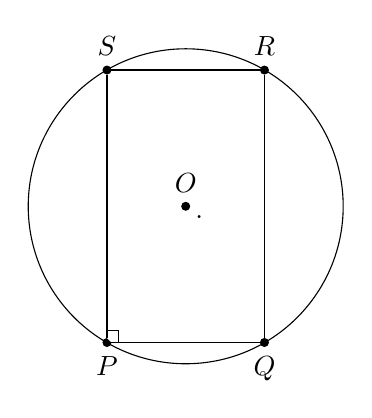
\begin{tikzpicture}
[scale =0.5,>=stealth,point/.style = {draw, circle, fill = black, inner sep = 1pt},]
\node (P) at (-2,-3.46)[point,label=below :$P$] {};
\node (Q) at (2,-3.46)[point,label=below :$Q$] {};
\node (R) at (2,3.46)[point,label=above :$R$] {};
\node (S) at (-2,3.46)[point,label=above :$S$] {};
\node (O) at (0,0)[point,label=above :$O$] {};
\draw (0,0) node [below right] {.} circle (4);
\draw (P)--(Q);
\draw (Q)--(R);
\draw (R)--(S);
\draw (S)--(P);

\tkzMarkRightAngle[fill=white!45,size=.3,mark=](S,P,Q)
\end{tikzpicture}
\end{document}
\end{center}
\item PQ = 2cm and PS = 4cm, radius = 4
\end{itemize}
\end{frame}
\begin{frame}
\begin{itemize}
\item \textbf{Calculation}
\end{itemize}
\begin{align*}
a = 2\\
c = 4\\
b = \sqrt{c^2} - a ^2\\
b = 3.46
\end{align*}
\end{frame}
\begin{frame}
\begin{figure}
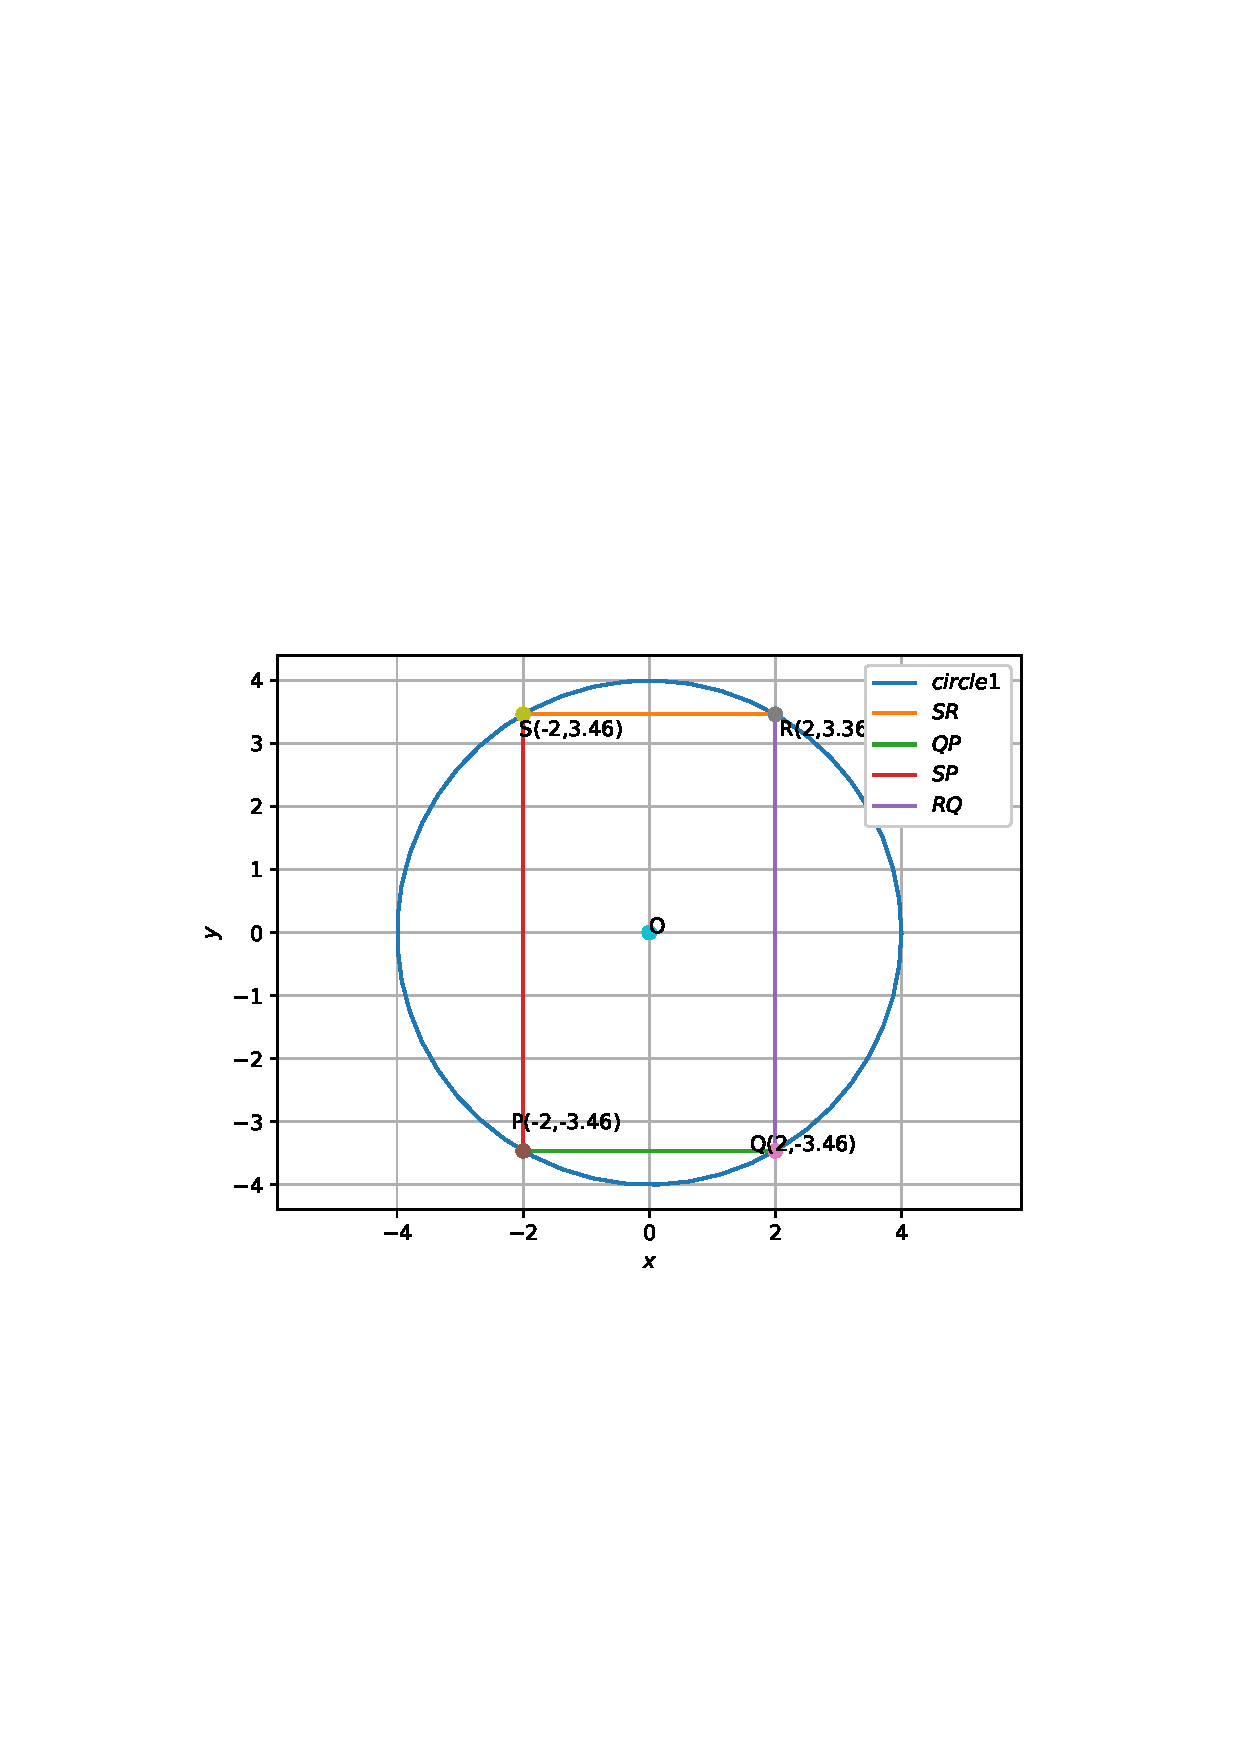
\includegraphics[scale=.4]{./CODES/quad/QUAD_P.png}
\end{figure}
\begin{itemize}
\item\url{https://github.com/pratibha444/GEOMETRY/blob/master/figs/CYCPA.tex}
\item\url{https://github.com/pratibha444/GEOMETRY/blob/master/CODES/quad/QUADP.py}
\end{itemize}
\end{frame}
\begin{frame}
\textbf{To prove} : PQRS is a rectangle\\
\textbf{Proof}: 
\begin{itemize}
\item $\angle$P = $\angle$R (opposite sides of parallelogram are equal)\\
\item $\angle$P + $\angle$R = 180$\degree$ (sum of opposite angles of a cyclic quadrilateral is 180$\degree$)\\

\item 2$\angle$P = 180$\degree$\\
\item$\angle$P = 90 $\degree$\\
Hence PQRS is a rectangle as in rectangle one angle is 90$\degree$\\
\end{itemize}
\end{frame}